\documentclass[12pt]{article}

\usepackage[margin=1in]{geometry} 
\usepackage[document]{ragged2e}

\usepackage{polski}
\usepackage[utf8]{inputenc} 
\usepackage{amssymb,amsmath}
\usepackage{ulem}

\usepackage{tikz}   
\usetikzlibrary{arrows}

\pagenumbering{gobble}

\begin{document}
\section*{Wykład 1, 21.02.2019 - $\mathbb{R}^2$ i $\mathbb{R}^3$}

\section{wektor}
\begin{minipage}[t]{0.48\textwidth}
    \underline{def}. (geometryczna) \\
        Para uporządkowana punktów w $\mathbb{R}^2 / \mathbb{R}^3 $. 
        Wektory mogą być swobodne lub zaczepione. My zajmujemy się wektorami swobodnymi. Przy czym:\\
        $ \overrightarrow{AB} = \overrightarrow{CD}$, jeśli mają jednakowe długości kierunki i zwroty. Gdzie:
        \begin{itemize} 
            \item długość - odległość z A do B
            \item kierunek - kierunek $ \overrightarrow{AB} $ to kierunek prostej AB (proste równoległe wyznaczają ten sam kierunek).
            \item zwrot - określone dla wektorów o tym samym kierunku. Gdy dwa wektory mają ten sam zwrot, gdy są skierowane w tę samą stronę.
        \end{itemize}
\end{minipage}
\hfill\vline\hfill
\begin{minipage}[t]{0.48\textwidth}
    \underline{def}. (algebraiczna)
    Wektor w $\mathbb{R}^2 \ (\mathbb{R}^3) $ to para (trójka) liczb rzeczywistych $\begin{pmatrix}x \\ y \end{pmatrix} (\begin{pmatrix}x \\ y \\ z\end{pmatrix})$.
    
    
    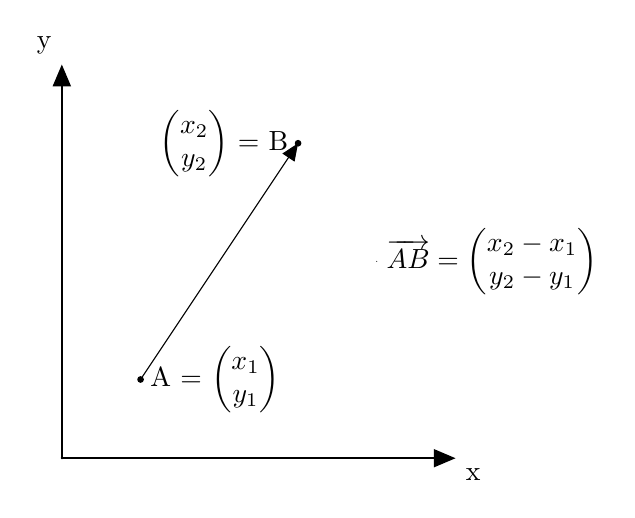
\begin{tikzpicture}[line cap=round,line join=round,>=triangle 45,scale=1,font=\normalsize] 
    \draw[thick,->] (0,0) -- (5,0) node[anchor=north west] {x};
    \draw[thick,->] (0,0) -- (0,5) node[anchor=south east] {y};
    
    \filldraw[black] (1,1) circle (1pt) node[anchor=west] {A = $\begin{pmatrix}x_1 \\ y_1 \end{pmatrix} $};
    \filldraw[black] (3,4) circle (1pt) node[anchor=east] {$\begin{pmatrix}x_2 \\ y_2 \end{pmatrix} $ = B};
    
    \draw[->] (1,1) -- (3,4);
    
    \filldraw[black] (4,2.5) circle (0pt) node[anchor=west] {$ \overrightarrow{AB} = \begin{pmatrix}x_2 - x_1 \\ y_2 - y_1 \end{pmatrix} $};
    
    
    \end{tikzpicture}
\end{minipage}

\vspace{10mm}
\uwave{\textbf{Konwencje}}
    \begin{itemize}
        \item $O = \begin{pmatrix}0 \\ 0 \end{pmatrix} $
        \item Utożasamiamy $\overrightarrow{OA} $ z punktem $A$.\\ \hspace{10mm} $\overrightarrow{OA} = A $
    \end{itemize}
\underline{\textbf{FAKT}}  $ \quad \overrightarrow{AB} = B - A $ \\
\vspace{2mm}
\underline{d-d.} $\quad \overrightarrow{AB} + \overrightarrow{AB} = \overrightarrow{OB}$ \\ 
\vspace{5mm}
\underline{Dodawanie wektorów} \\
\begin{minipage}[c]{0.33\textwidth}
    \vspace{3mm}
    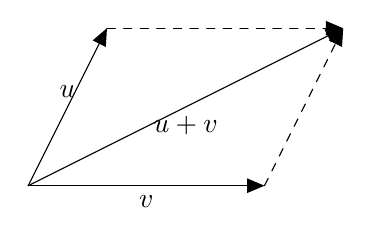
\begin{tikzpicture}[line cap=round,line join=round,>=triangle 45,scale=1,font=\normalsize] 
        \draw[->] (0,0) -- (1,2) node[midway,above] {$u$};
        \draw[->] (0,0) -- (3,0) node[midway,below] {$v$};
        \draw[dashed,->] (1,2) -- (4,2);
        \draw[dashed,->] (3,0) -- (4,2);
        \draw[->] (0,0) -- (4,2) node[midway,below] {$u+v$};
    \end{tikzpicture} \\
    Zasada równoległboku
\end{minipage}%
\begin{minipage}[c]{0.33\textwidth}
    \vspace{3mm}
    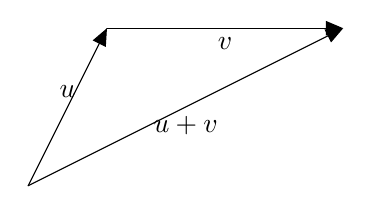
\begin{tikzpicture}[line cap=round,line join=round,>=triangle 45,scale=1,font=\normalsize] 
        \draw[->] (0,0) -- (1,2) node[midway,above] {$u$};
        \draw[->] (1,2) -- (4,2) node[midway,below] {$v$};
        \draw[->] (0,0) -- (4,2) node[midway,below] {$u+v$};
    \end{tikzpicture} \\
    \vspace{3mm}
    Zasada trójkąta
\end{minipage}%
\begin{minipage}[c]{0.33\textwidth}
    \vspace{8mm}
    $\begin{pmatrix}x\\ y\end{pmatrix} + \begin{pmatrix}x'\\ y'\end{pmatrix} = \begin{pmatrix}x+x'\\ y+y'\end{pmatrix}$ \\
    \vspace{8mm}
    algebraicznie
\end{minipage}

\end{document}
